\documentclass{article}
\usepackage{tikz, comment}
\usepackage{pifont}
\usepackage{fontspec, pgfplots}
\usetikzlibrary{arrows, decorations.markings, decorations.pathreplacing}
\begin{comment}
:Title: Not defined yet
:Tags: properties of equality, equation rules;absolute value rules;equivalence properties of equality;inequality rules;joint variation, jointly proportional
:Prob: 0.6224;0.5949;0.5741;0.5661;0.5541
:Author: Prof.Hu Ji-shan, HKUST
:Slug: No name yet

Description Here.........
\end{comment}
\begin{document}\centering 

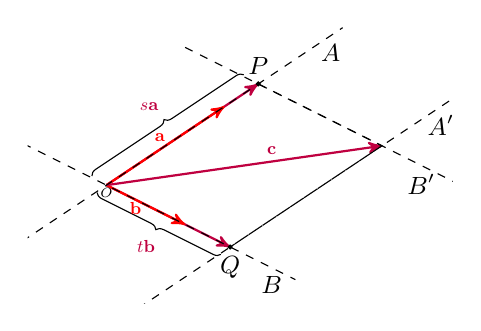
\begin{tikzpicture}[>=latex,xscale=.5*1, yscale=.5*1][font=\sf\small] 

%\draw[xstep=1cm,ystep=1cm,color=gray!80] (-2, -3) grid (8, 4);

    	\foreach \x in {}
     		\draw (\x,2pt/8) -- (\x,-2pt/8)
			node[anchor=north] {\tiny$\x$}
			;

    	\foreach \x in {}
     		\draw (\x,2pt/1) -- (\x,-2pt/1)
			node[anchor=south] {\tiny$\x$}
			;
    	\foreach \y in {}
     		\draw (-2pt/1,\y) -- (2pt/1,\y)
			node[anchor=east] {\tiny $\y$}
			;

%\draw[->] (-2, 0) -- (8, 0)node[below] {$x$} ;
%\draw[->] (0, -3) -- (0, 4)node[left] {$y$} ;

\clip[] (-2, -3) rectangle (8.8, 4);

\draw[purple, thick, ->, >=stealth'] (0, 0) -- ({3*9/7}, {2*9/7});

\draw [decoration={brace,raise=4},decorate, xshift=-6] 
(0, 0) -- ({3*9/7}, {2*9/7})node[purple, fill=white, midway, pos=0.5, xshift=-9, yshift=10, scale=0.7]{$s{\bf a}$};

\draw[red, thick, opacity=1, ->, >=stealth'] (0, 0) -- (3, 2)node[opacity=1, left, midway, pos=0.6, xshift=-2, yshift=0, scale=0.7]{${\bf a}$};

\draw[purple, thick, ->, >=stealth'] (0, 0) -- ({2*11/7}, {-1*11/7});

\draw [decoration={brace,raise=3, mirror},decorate, xshift=-4] 
(0, 0) -- ({2*11/7}, {-1*11/7})node[purple, fill=white, midway, pos=0.5, xshift=-6, yshift=-11, scale=0.7]{$t{\bf b}$};

\draw[red, thick, ->, >=stealth'] (0, 0) -- (2, -1)node[opacity=1, left, midway, pos=0.6, xshift=-2, yshift=0, scale=0.7]{${\bf b}$};

\draw[purple, thick, ->, >=stealth'] (0, 0) -- (7, 1)node[above, midway, pos=0.6, xshift=0, yshift=0, scale=0.7]{${\bf c}$};

\draw[dashed] ({3*(-2)}, {2*(-2)}) -- ({3*2}, {2*2});
\draw[dashed] ({3*(-3)+7}, {2*(-3)+1}) -- ({3*3+7}, {2*3+1});

\draw[dashed] ({2*(-2)}, {-1*(-2)}) -- ({2*2.4}, {-1*2.4});
\draw[dashed] ({2*(-2.5)+7}, {-1*(-2.5)+1}) -- ({2*3+7}, {-1*3+1});

\draw[dashed] ({3*9/7}, {2*9/7})--(7, 1)--({2*11/7}, {-1*11/7});

\node[below] at ({3*1.9}, {2*1.9}) {$A$};
\node[below] at ({3*0.5+7}, {2*0.5+1}) {$A'$};

\node[below] at ({2*2.1}, {-1*2.1}) {$B$};
\node[below] at ({2*0.5+7}, {-1*0.5+1}) {$B'$};

\draw[fill] ({3*9/7}, {2*9/7}) circle(0.05)node[above]{$P$};
\draw[fill] ({2*11/7}, {-1*11/7}) circle(0.05)node[below]{$Q$};

\node[scale=0.7] at (0/1, -0.2/1) {\scriptsize$O$};

\end{tikzpicture}
\end{document}